\begin{frame}
    \frametitle{Performance Measures - Steady state vector}
    
    \tiny
    \begin{equation*}
        Q = 
        \begin{blockarray}{ccccccc}
            (0, 0) & (0, 1) & (0, 2) & & (2, 3) & (2, 4) & \\
            & & & & & & & \\
            \begin{block}{(cccccc)c}
                -\lambda_1 - \lambda_2 & \lambda_1 + \lambda_2 & 0 & \dots & 0 & 0 & (0,0) \\
                \mu & -\mu - \lambda_1 - \lambda_2 & \lambda_1 + \lambda_2 & \dots & 0 & 0 & (0,1) \\
                0 & 2\mu & -2\mu - \lambda_1 - \lambda_2 & \dots & 0 & 0 & (0,2) \\
                \vdots & \vdots & \vdots & \ddots & \vdots & \vdots \\
                0 & 0 & 0 & \dots & -\lambda_1 - 3\mu & \lambda_1 & (2,3) \\
                0 & 0 & 0 & \dots & 3\mu & -3\mu & (2,4) \\
            \end{block}
        \end{blockarray}    
    \end{equation*}

    \normalsize
    \begin{equation*}
        \frac{d \pi}{dt} = \pi Q = 0 
    \end{equation*}

    \begin{equation*}
        \pi = \left[
            \pi_{(0,0)}, \pi_{(0,1)}, \pi_{(0,2)}, \dots, \pi_{(2,3)}, \pi_{(2,4)}
        \right], \hspace{1cm} \sum \pi_i = 1
    \end{equation*}

\end{frame}


\begin{frame}
    \frametitle{Performance Measures - Waiting time}
    \centering
    \begin{equation}
        W = \frac{\lambda_1 P_{L'_1}}{\lambda_2 P_{L'_2} + \lambda_1 P_{L'_1}} W^{(1)} 
        + \frac{\lambda_2 P_{L'_2}}{\lambda_2 P_{L'_2} + \lambda_1 P_{L'_1}} W^{(2)}
    \end{equation}

    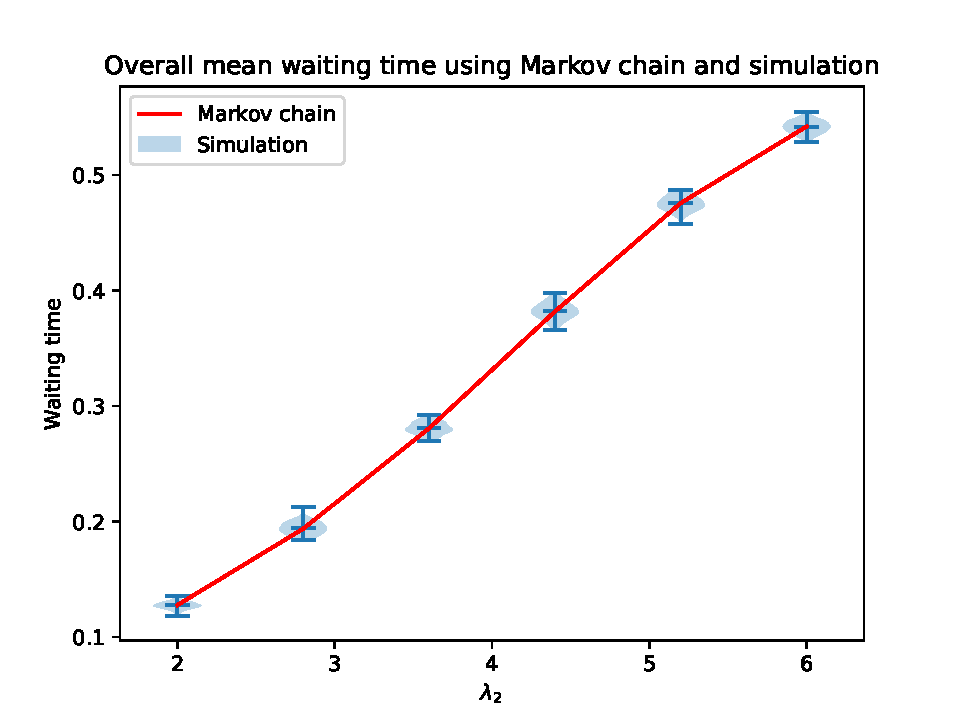
\includegraphics[scale=0.5]{Bin/waiting_overall_comparison.pdf}
\end{frame}


\begin{frame}
    \frametitle{Performance Measures - Blocking time}
    \centering
    \begin{equation}
        B = \frac{\sum_{(u,v) \in S_A^{(2)}} \pi_{(u,v)} \; 
        b(u,v)}{\sum_{(u,v) \in S_A^{(2)}} \pi_{(u,v)}}
    \end{equation}

    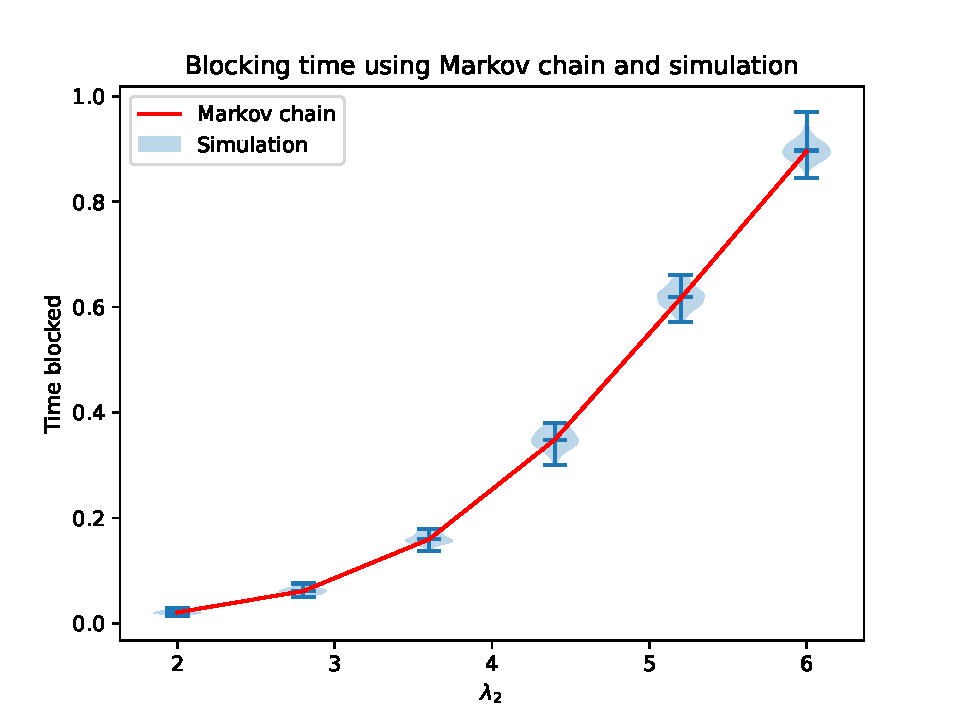
\includegraphics[scale=0.5]{Bin/blocking_comparison.pdf}
\end{frame}


\begin{frame}
    \frametitle{Performance Measures - Proportion within time}
    \centering
    
    \small
    \begin{equation}
        P(X < t) = \frac{\lambda_1 P_{L'_1}}{\lambda_2 P_{L'_2}+\lambda_1 P_{L'_1}} 
        P(X^{(1)} < t) + \frac{\lambda_2 P_{L'_2}}{\lambda_2 P_{L'_2} + 
        \lambda_1 P_{L'_1}}P(X^{(2)} < t) 
    \end{equation}
    \normalsize

    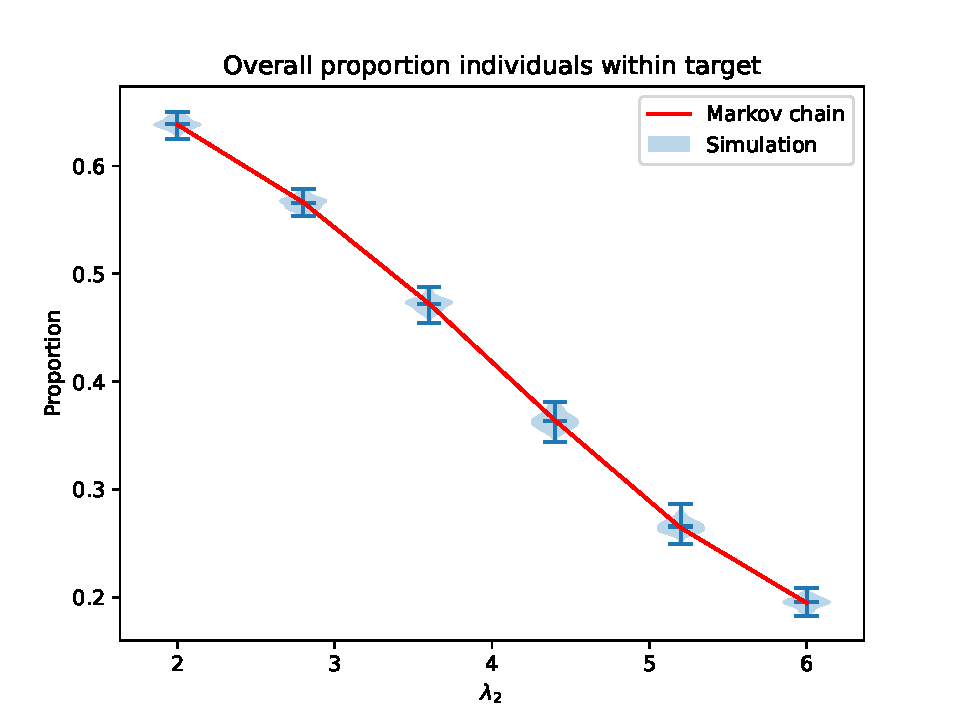
\includegraphics[scale=0.5]{Bin/proportion_overall_comparison.pdf}

\end{frame}